\documentclass{article}

\usepackage{graphicx}
\usepackage{authblk}
\usepackage{listings}
\usepackage{xcolor}
\usepackage[a4paper,
            bindingoffset=0.2in,
            left=0.5in,
            right=0.5in,
            top=0.5in,
            bottom=0.5in,
            footskip=.25in]{geometry}

\definecolor{mGreen}{rgb}{0,0.6,0}
\definecolor{mGray}{rgb}{0.5,0.5,0.5}
\definecolor{mPurple}{rgb}{0.58,0,0.82}
\definecolor{backgroundColour}{rgb}{0.95,0.95,0.92}

\lstdefinestyle{CStyle}{
    backgroundcolor=\color{backgroundColour},   
    commentstyle=\color{mGreen},
    keywordstyle=\color{magenta},
    numberstyle=\tiny\color{mGray},
    stringstyle=\color{mPurple},
    basicstyle=\footnotesize,
    breakatwhitespace=false,         
    breaklines=true,                 
    captionpos=b,                    
    keepspaces=true,                 
    numbers=left,                    
    numbersep=5pt,                  
    showspaces=false,                
    showstringspaces=false,
    showtabs=false,                  
    tabsize=2,
    language=C
}


\title{Lab Exercise 3: Selection Statements (if/else if and switch)}
\author{Cody Raposa}
\affil{ELEC2850 Microcontrollers Using C Programming}

\begin{document}
\maketitle
\begin{flushleft}
  \section{Problem Statement}
  Given a table of boiling points of several substances, create a program that gets the user's \
  boiling point of their fluid (in \textdegree Celcius) and tells the user what substace their fluid is \
  as long as the substance is within 5\% of the given boiling point. When the substance is unkown, let the user know that.
  \begin{table}[h]
    \caption{Expected boiling points of substances.}
    \begin{center}
      \begin{tabular}{ c c }
        Substance & Normal boiling point (\textdegree C) \\
        \hline
        Water     & 100                                  \\
        Mercury   & 357                                  \\
        Copper    & 1187                                 \\
        Silver    & 2193                                 \\
        Gold      & 2660                                 \\
        \hline
      \end{tabular}
    \end{center}
  \end{table}
  %\section{Assumptions}
  %\section{Algorithm}
  \section{Analysis}
  \subsection{Inputs}
  Boiling Point of fluid (float)
  \subsection{Outputs}
  Fluid with boiling point +- 5\% of given boiling point (string)
  %\subsection{Formulas}
  %\section{Pseudocode}
  \newpage
  \section{Flowchart}
  \begin{figure}[!h]
    \begin{centering}
      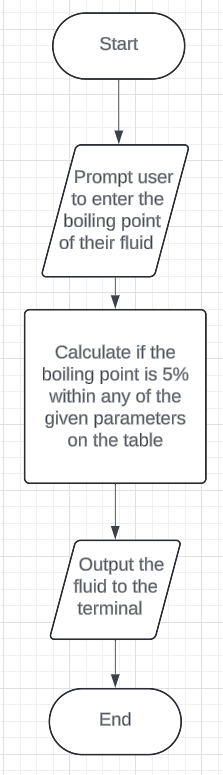
\includegraphics[scale=1]{Q1_flowchart.png}
      \caption{Flowchart for Question 1}
    \end{centering}
  \end{figure}
  \newpage
  \section{Output}
    \begin{figure}[!h]
      \begin{centering}
        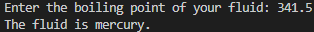
\includegraphics[scale=1]{Q1_p1.png}
        \caption{Output with 341.5 degrees as boiling point}
      \end{centering}
    \end{figure}
    \begin{figure}[!h]
      \begin{centering}
        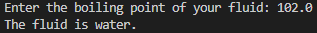
\includegraphics[scale=1]{Q1_p2.png}
        \caption{Output with 102 degrees as boiling point}
      \end{centering}
    \end{figure}
  You cannot handle this problem with a switch case as you cannot use ranges in a switch case.
  \section{Code}
  \lstinputlisting[style=CStyle]{Q1.c}
  \newpage
  \section{Part 2 Problem Statement}
  Use a switch to create one promgram the performs the following operations:
  \begin{itemize}
    \item Absolute value
    \item Maximum
    \item Minimum
    \item Sum
    \item Difference
    \item Square
  \end{itemize}
  \section{Analysis}
  \subsection{Inputs}
  What action the user wants to perform (char)
  The numbers the user wants the program to perform the action on (float)
  \subsection{Outputs}
  The result of the action (float)
  \subsection{Formulas}
  \begin{itemize}
    \item Absolute value: $|x|$
    \item Maximum: $\max(x, y)$
    \item Minimum: $\min(x, y)$
    \item Sum: $x + y$
    \item Difference: $x - y$
    \item Square: $x^2$
  \end{itemize}
  \newpage
  \section{Flowchart}
  \begin{figure}[!h]
    \begin{centering}
      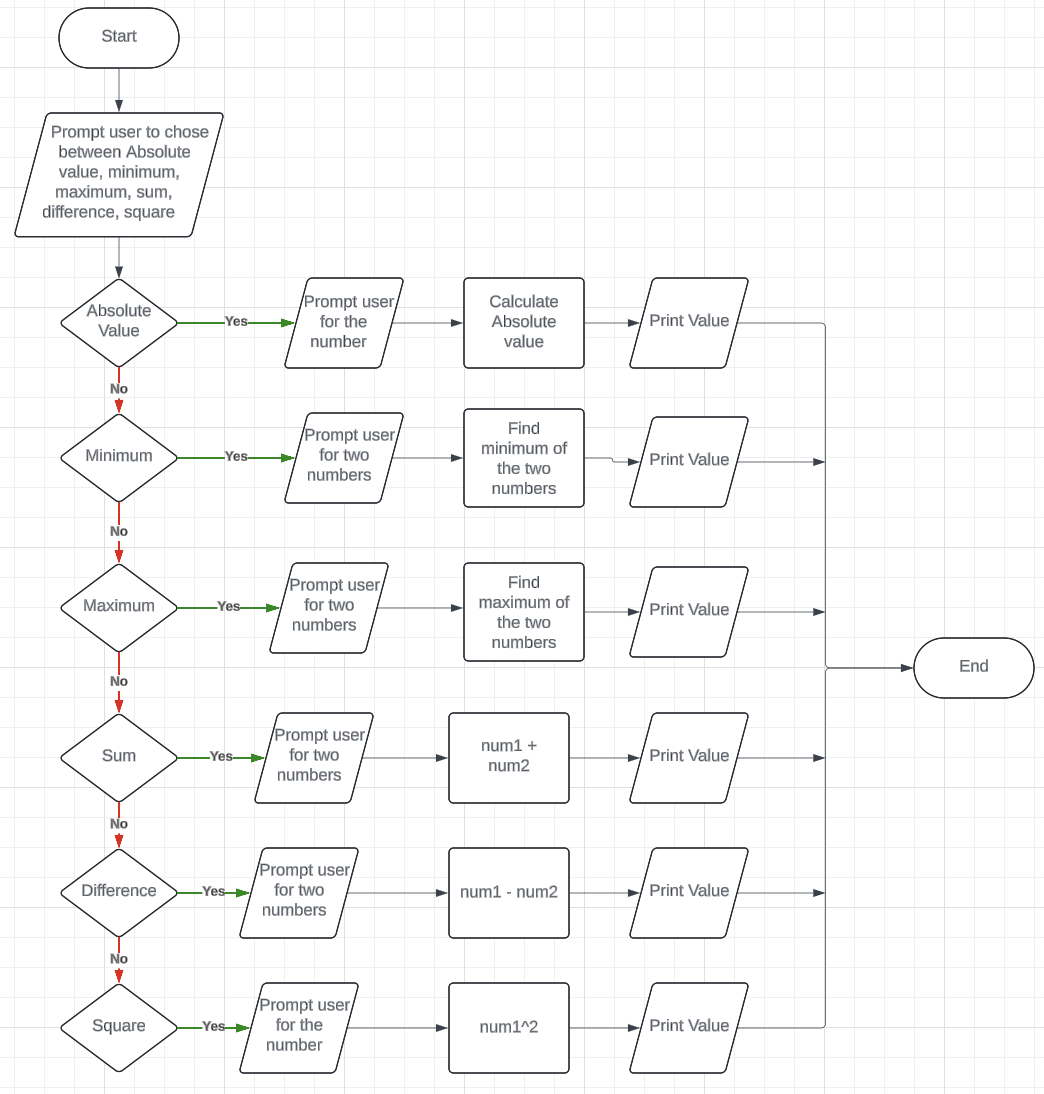
\includegraphics[scale=0.55]{Q2_flowchart.png}
      \caption{Flowchart for Question 2}
    \end{centering}
  \end{figure}
  \newpage
  \section{Output}
  \begin{figure}[!h]
    \begin{centering}
      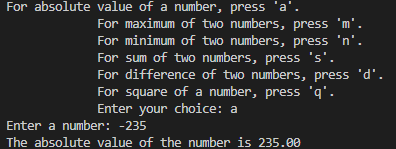
\includegraphics[scale=1]{Q2_p1.png}
      \caption{Test case for Absolute value}
    \end{centering}
  \end{figure}
  \begin{figure}[!h]
    \begin{centering}
      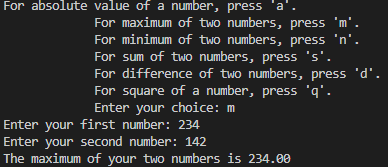
\includegraphics[scale=1]{Q2_p2.png}
      \caption{Test case for Maximum}
    \end{centering}
  \end{figure}
  \begin{figure}[!h]
    \begin{centering}
      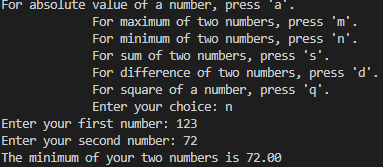
\includegraphics[scale=1]{Q2_p3.png}
      \caption{Test case for Minimum}
    \end{centering}
  \end{figure}
  \begin{figure}[!h]
    \begin{centering}
      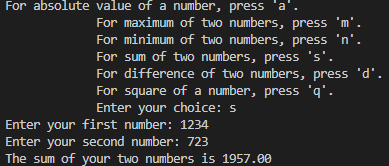
\includegraphics[scale=1]{Q2_p4.png}
      \caption{Test case for Sum}
    \end{centering}
  \end{figure}
  \begin{figure}[!h]
    \begin{centering}
      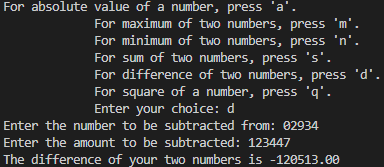
\includegraphics[scale=1]{Q2_p5.png}
      \caption{Test case for Difference}
    \end{centering}
  \end{figure}
  \begin{figure}[!h]
    \begin{centering}
      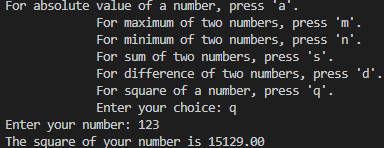
\includegraphics[scale=1]{Q2_p6.png}
      \caption{Test case for Square}
    \end{centering}
  \end{figure}
  \begin{figure}[!h]
    \begin{centering}
      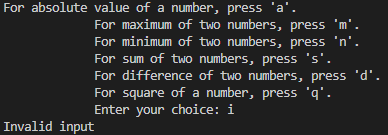
\includegraphics[scale=1]{Q2_p7.png}
      \caption{Invalid input}
    \end{centering}
  \end{figure}
  \newpage
  \newpage
  \section{Code}
  \lstinputlisting[style=CStyle]{Q2.c}
\end{flushleft}
\end{document}